The user should be able to make a taxi request from the web application and the mobile application. If the request comes from the web application, the user has to tell the system the origin and the destination of the ride, otherwise they can be taken using the GPS of the mobile application.
After the user makes the request, he receives a notification from the system with the identifier of the taxi and the possible arrival time of the taxi.
Once the request is sent to the system, the system has to send it to the first taxi driver available, who can accept or deny the request.

\subparagraph{Use case}
\noindent
    \begin{center}
        \begin{longtable}{| l | p{0.6\textwidth} |}
            \hline
            Actor & Passenger \\
            \hline
            Goal & Goal~\ref{g-manage}
            \\
            \hline
            Input condition & A user chooses to make a taxi request from his account page \\
            \hline
            Event Flow & 
                \begin{enumerate}
                	\item The user makes a request of a taxi inserting all the required information in the application page;
                	\item The user sends the request to the system using the "Send request" button.
            	\end{enumerate}
            \\
            \hline
            Output condition & The user after a while receives the confirmation of the request. \\
            \hline
            Exception & 
            \begin{itemize}
                \item There are no available taxi in the area;
                \item The user waits for the confirmation for more than 10 minutes;
                \item When ten taxi drivers refuse the reservation, it is canceled.
            \end{itemize} \\
            \hline
        \end{longtable}
    \end{center}

\subparagraph{Functional requirements}
\noindent
	\begin{itemize}
		\item The origin and the destination must be valid [View assumptions]. They must be within 10Km from the city boundaries.
		\item If the request is made using the web application, the system shall be provided with the passenger location inserted directly by the user.
		\item If the request is made using the mobile application, the system can use the GPS position to identify the user location.
		\item If the GPS is not available, the system tells the passenger to insert the correct origin location for the taxi ride.
		\item If the origin and/or the destination are not specified (neither from GPS nor from the user insertion), the user can not proceed to send the request.
		\item If a request is not accepted by a taxi driver, it is passed to the next driver in the queue of the city zone.
	\end{itemize}
	
\begin{figure}[H]
    \centering
    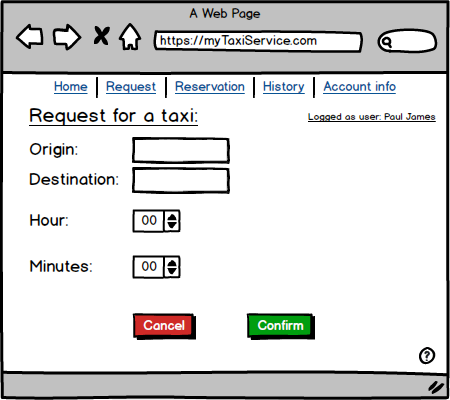
\includegraphics[width=\textwidth]{./Mockups/RequestWeb.png}
    \caption{Request page of the web application}
\end{figure}